\documentclass[a4paper]{article}

%% Language and font encodings
\usepackage[english]{babel}
\usepackage[utf8]{inputenc}
\usepackage[T1]{fontenc}
\usepackage{authblk}
\usepackage{booktabs}
\usepackage{ae,aecompl}
%% Sets page size and margins
\usepackage[a4paper,top=3cm,bottom=2cm,left=3cm,right=3cm,marginparwidth=1.75cm]{geometry}

%% Useful packages
\usepackage{pgfplots}
\pgfplotsset{compat=1.12}
\usepackage[group-separator={,}]{siunitx}
\usepackage{amsmath}
\usepackage{wrapfig}
\usepackage{amsthm}
\usetikzlibrary{arrows,automata}
\usepackage{algpseudocode}
\usepackage{graphicx}
\usepackage{algorithm}
\usepackage{breqn}
\usepackage{algpseudocode}
\usepackage{float}
\usepackage{tikz}
\usepackage{pifont}% http://ctan.org/pkg/pifont
\newcommand{\cmark}{\ding{51}}%
\newcommand{\xmark}{\ding{55}}%
\usepackage{eufrak}
\usepackage{caption}
\usepackage{subcaption}
\usepackage{listings}
\usepackage[toc,page]{appendix}
\usepackage{color}
\definecolor{lightgray}{rgb}{.9,.9,.9}
\definecolor{darkgray}{rgb}{.4,.4,.4}
\definecolor{purple}{rgb}{0.65, 0.12, 0.82}
\floatname{algorithm}{Procedure}
\renewcommand{\algorithmicrequire}{\textbf{Input:}}
\renewcommand{\algorithmicensure}{\textbf{Output:}}

\lstdefinelanguage{JavaScript}{
	keywords={typeof, contract, struct, new, true, false, catch, function, return, null, catch, switch, var, if, in, while, do, else, case, break},
	keywordstyle=\color{blue}\bfseries,
	ndkeywords={class, export, boolean, throw, implements, import, this},
	ndkeywordstyle=\color{darkgray}\bfseries,
	identifierstyle=\color{black},
	sensitive=false,
	comment=[l]{//},
	morecomment=[s]{/*}{*/},
	commentstyle=\color{purple}\ttfamily,
	stringstyle=\color{red}\ttfamily,
	morestring=[b]',
	morestring=[b]"
}

\lstset{
	language=JavaScript,
	backgroundcolor=\color{lightgray},
	extendedchars=true,
	basicstyle=\footnotesize\ttfamily,
	showstringspaces=false,
	showspaces=false,
	numbers=left,
	numberstyle=\footnotesize,
	numbersep=9pt,
	tabsize=2,
	breaklines=true,
	showtabs=false,
	captionpos=b
}

\usepackage{graphicx}
\usepackage[
n,
operators,
advantage,
sets,
adversary,
landau,
probability,
notions,	
logic,
ff,
mm,
primitives,
events,
complexity,
asymptotics,
keys]{cryptocode}
\usepackage[colorinlistoftodos]{todonotes}
\usepackage[colorlinks=true, allcolors=blue]{hyperref}

\theoremstyle{definition}
\newtheorem{definition}{Definition}[section]

\newcommand{\Mod}[1]{\ (\mathrm{mod}\ #1)}

\def\bitcoinA{%
	\leavevmode
	\vtop{\offinterlineskip %\bfseries
		\setbox0=\hbox{B}%
		\setbox2=\hbox to\wd0{\hfil\hskip-.03em
			\vrule height .3ex width .15ex\hskip .08em
			\vrule height .3ex width .15ex\hfil}
		\vbox{\copy2\box0}\box2}}

\DeclareMathOperator{\EX}{\mathbb{E}}% expected value
\providecommand{\keywords}[1]{\textbf{\textit{Keywords:}} #1}

\renewcommand{\lstlistingname}{Figure}% Listing -> Algorithm
\renewcommand{\lstlistlistingname}{List of \lstlistingname s}% List of Listings -> List of Algorithms

\newcommand{\smallsim}{\smallsym{\mathrel}{\sim}}

\makeatletter
\newcommand{\smallsym}[2]{#1{\mathpalette\make@small@sym{#2}}}
\newcommand{\make@small@sym}[2]{%
	\vcenter{\hbox{$\m@th\downgrade@style#1#2$}}%
}
\newcommand{\downgrade@style}[1]{%
	\ifx#1\displaystyle\scriptstyle\else
	\ifx#1\textstyle\scriptstyle\else
	\scriptscriptstyle
	\fi\fi
}
\makeatother


\title{MixEth: efficient, trustless coin mixing service for Ethereum}
\author[1]{István András Seres}
\author[1]{Dániel A. Nagy}
\author[2]{Chris Buckland}
\author[1]{Péter Burcsi}
\affil[1]{Department of Computer Algebra, Eötvös Loránd University}
\affil[2]{King's College London}
\begin{document}
\maketitle

\begin{abstract}
Cryptocurrencies enable users to transact pseudonymously with each other without relying on trusted parties or intermediaries. These transactions are recorded in an immutable, publicly verifiable ledger. Due to the ledger's transparent nature, privacy is notably reduced. If the link between users' public key and their physical identity is exposed, their pseudonymity is lost. One way to increase users' privacy is to deploy coin mixing services. In this paper, we present MixEth, which is a trustless coin mixing service. MixEth is more efficient than any current proposed trustless coin tumbler. It requires at most only $3$ on-chain transactions per user and $1$ off-chain message. It achieves strong notions of anonymity and is able to resist denial-of-service attacks. Furthermore the underlying protocol can also be used to efficiently shuffle ballots and cyphertexts in a trustless and decentralized manner.     
\end{abstract}
\keywords{Cryptography, Verifiable shuffle, Ethereum, Privacy, Coin mixer, State Channel}

\section{Introduction}
One of the methods to increase cryptocurrency users' privacy is coin mixing or tumbling. This technique provides \textit{k-anonymity} or \textit{plausible deniability}. The idea is that $k$ users deposit $1$ coin each and then in the course of a coin shuffling protocol either a centralized trusted third party or a smart contract mixes the coins and redistributes them to designated fresh public keys. This powerful technique gives users superior privacy and anonymity since their newly received coins can not be linked to them.

Several coin mixing protocols were proposed in the literature both centralized (\cite{bonneau2014mixcoin}, \cite{valenta2015blindcoin}, \cite{heilman2017tumblebit}) and decentralized (\cite{maxwell2013coinjoin}, \cite{ruffing2014coinshuffle}, \cite{miximus2018}, \cite{meiklejohn2018mobius}, \cite{bissias2014sybil}). A major drawback of centralized coin mixing is that the availability of the tumbler is entirely dependent on the trusted party and in most cases theft prevention can not be guaranteed (\cite{bonneau2014mixcoin}, \cite{valenta2015blindcoin}). On the other hand decentralized tumblers achieve availability, theft prevention and satisfy strong notions of anonymity although they are considerably heavier computationally. 

The two major techniques to provide decentralized mixing services for Ethereum are Möbius, a ring-signature-based solution \cite{meiklejohn2018mobius} and Miximus, a zkSNARK-based proposal \cite{miximus2018}. Both of them require usage of a large amount of gas to withdraw funds, which could be prohibitive for many use cases. Möbius requires $\num[group-separator={,}]{335714}n$ gas ($n$ is the ring size) while Miximus consumes $\num[group-separator={,}]{1903305}$ gas to verify a zkSNARK proof \cite{miximus2018gascost}.

\textbf{Our contributions.} In this paper, we present a trustless and efficient mixing protocol for Turing-complete blockchains. To show the practicality of the protocol, we introduce MixEth, a privacy-enhancing protocol and a practical tool for Ethereum. MixEth overcomes the above mentioned efficiency issues of an Ethereum-based coin-mixer while retaining the strong notions of anonymity, mixer availability and theft prevention already achieved by previous proposals (\cite{meiklejohn2018mobius},\cite{miximus2018}). MixEth requires as few off-chain messages and on-chain transactions as Möbius and Miximus, meanwhile it burns significantly less gas.

We also implement MixEth in a state channel to leverage the scalability and instant finality of off-chain scaling solutions.


\section{Background}
\subsection{Notations}
Let $[]$ denote the empty tuple. For a tuple $t=(x_1,\dots,x_n)$ we denote $t[x_i]$ as the value stored at $x_{i}$. The cardinality of a finite set $X$ is denoted as $|X|$. In the following let $\lambda \in \mathbb{N}$ be the security parameter and its unary representation is $1^{\lambda}$. If $x$ is uniformly randomly sampled from a set $A$ we write $x\stackrel{\$}{\leftarrow}A$. The symmetric group of degree $n$ is written as ${S}_n$. In a cyclic group $\mathbb{G}$, the standardized generator is denoted as $G$ and we use the additive notation. Secret keys and public keys are denoted as $sk$ and $pk$ respectively (or often times $s$ and $sG$), while the user the corresponding key belongs to is indicated in subscript. Let $PK_{i}$ denote the set of public keys belonging to receivers at a particular shuffling round $i$.

\subsection{Cryptographic keys in Ethereum}
Ethereum uses Elliptic Curve Cryptography (ECC) to secure users' funds. More specifically, it uses the secp256k1 curve, the same one as used in Bitcoin. If a user wants to create an Ethereum address, first they need to generate a secret key  $s\stackrel{\$}{\leftarrow}\mathbb{Z}_n$, where $n$ is the order of secp256k1 over a finite prime field $\mathbb{F}_{p}$. The corresponding public key will be $sG$. Note, that any multiples of $G$ is also a generator of curve points since $n$, the order of the group is also a prime. Accounts in Ethereum are identified by their addresses which can be obtained by taking the right most 20 bytes of the Keccak hashed public key \cite{wood2014ethereum}. 
    
\subsection{Decision Diffie-Hellman Problem and Chaum-Pedersen Protocol}

The Decision Diffie-Hellman assumption (DDH) is a standard cryptographic hardness assumption which underlies the security of many cryptographic protocols. Roughly speaking DDH states that no efficient algorithm can distinguish between the two distributions $(aG, bG, abG)$ and $(aG, bG, cG)$, where $a,b,c\stackrel{\$}{\leftarrow}\mathbb{Z}_{|\mathbb{G}|}$. It is believed that the DDH assumption holds for elliptic curves with prime order over a prime field with large embedding factor \cite{boneh1998decision}, specifically DDH holds for the secp256k1 curve used in Ethereum.

The language $\mathcal{L}_{DDH}$ is defined to be the set of all tuples $(G,aG,bG,abG)$ where $G\in \mathbb{G}$ is of order prime $q$. The Chaum-Pedersen protocol enables a prover $\mathcal{P}$ to prove to a verifier $\mathcal{V}$ that $(G,A,B,C)\in\mathcal{L}_{DDH}$ in zero-knowledge for groups of prime order \cite{chaum1992wallet}. The protocol is organized as follows:

\begin{enumerate}
	\item $\mathcal{V}$: $s\stackrel{\$}{\leftarrow}\mathbb{Z}_q$, then sends $commit(s)$ 
	\item $\mathcal{P}$: $r\stackrel{\$}{\leftarrow}\mathbb{Z}_q$, then sends $y_1=rG$, $y_2=rB$.
	\item $\mathcal{V}$ opens commitment by sending $s$
	\item $\mathcal{P}$ sends $z=r+as \Mod{q}$
	\item $\mathcal{V}$ checks $zG=y_{1}+sA \Mod{q} \land zB=y_{2}+sC \Mod{q}$
\end{enumerate} 
Note that in the following a non-interactive version of this protocol will only be considered. This can be achieved by applying the Fiat-Shamir heuristic. 

\subsection{ECDSA with arbitrary generator element}
Elliptic Curve Digital Signature Algorithm (ECDSA) is a key component of MixEth. ECDSA is widely deployed in practice, where in most cases signatures are generated and verified with respect to a fixed generator element of the underlying group \cite{fersch2016provable}. Since all generators are equal from a security point of view, a single generator element is usually fixed in order to promote standardization and assist usability.

However, in MixEth, we require the use of arbitrary generator elements. Such an extension is needed for withdrawing funds from the mixer as the shuffled public keys remain public keys with respect to non-standardized generator elements. Therefore the usual $\sig$ and $\verify$ algorithms for signing and verifying messages require an additional parameter $G^{'}$, which is not necessarily the standardized generator element. Key generation algorithm works as usual $(pk,sk)\stackrel{\$}{\leftarrow}\kgen(1^{\lambda})$, on the other hand $\sigma\stackrel{\$}{\leftarrow}\sig(G^{'},sk,m)$ and  $0/1\leftarrow \verify(G^{'},pk,\sigma, m)$ accept new generators.

\section{Security goals} \label{securitygoals}
We are aiming to achieve and prove the same notions of security as the ones defined in \cite{meiklejohn2018mobius}, namely anonymity, availability and theft prevention. These notions of anonymity, availability and theft prevention were introduced in \cite{meiklejohn2018mobius}.

We are going to assume that at most $n-2$ recipients are malicious ($n$ is the number of recipients). Otherwise, no meaningful notion of security can be achieved. Furthermore we presume that recipients are on-line during the entire course of mixing in order to be able to monitor and potentially challenge any incorrect shuffle. Finally we assume that honest participants will always exercise their rights to shuffle and they do not disclose any private information used in their shuffles.

\begin{itemize}
	\item \textbf{Anonymity}: \textit{Sender} anonymity is achieved if an adversary can not determine to whom honest senders are sending funds, assuming that honest senders' deposits are indistinguishable. \textit{Recipient} anonymity is achieved if honest recipients withdrawal transactions are indistinguishable. 
	\item \textbf{Availability}: means that honest recipients can always withdraw their assets from the mixer, even if all participants are compromised. Adversary $\adv$ wins the availability security game if they manage to get the tumbler into a state where honest recipient can not withdraw their funds.
	\item \textbf{Theft prevention}: We would like to ensure that neither coins can be withdrawn twice, nor withdrawn by anyone other but the intended recipient.
\end{itemize}
\section{MixEth}
\subsection{Initializing the tumbler and depositing period}

A MixEth contract is deployed on the Ethereum blockchain at $id_{contract}$ address and is initialized with the $amt$ parameter which denotes the denomination of ether to be mixed.
Every sender must deposit exactly $amt$ ether to a specific public key. Deposits with incorrect ether value or invalid public key are rejected. Public keys in subsequent deposit transactions are written into the $initPubKeys[]$ array.   

\subsection{Shuffling period}
After the depositing round the shuffling and challenging rounds alternate in turn. Each shuffling round is followed by a challenging round where the correctness of the preceding shuffle can be challenged by anyone. If a challenge is accepted, then shuffler's deposit is lost, their shuffle is discarded and shuffling continues from the set of public keys prior to the discarded shuffle. In the course of a shuffle an honest shuffler multiplies all the public keys with a secret multiplier $c$ and then permutes the transformed public keys. This shuffling is done off-chain, then the shuffler commits to $c$ by sending back to MixEth the new shuffling accumulated constant and the shuffled public keys. This allows anyone to verify the shuffle and, if required, submit a challenge during the succeeding challenge round.

\begin{algorithm}[H]
	\caption{Off-chain public key shuffling algorithm for the $i$th shuffling round}\label{shufflingoffchain}
	\begin{algorithmic}[H]
		\State $PK_{i} \gets []
		,c\stackrel{\$}{\leftarrow}\mathbb{Z}_n,\pi\stackrel{\$}{\leftarrow}S_{|PK_{i-1}|}$
		\State $C^{*}_{i-1}\leftarrow read\ from\ MixEth\ contract$
		\State $PK_{i-1}\leftarrow read\ from\ MixEth\ contract\ the\ current\ sequence\ of\ shuffled\ public\ keys$
		\For{$j=0;j<|PK_{i-1}|;j++$}
		\State $PK_{i}[\pi(j)]=c*PK_{i-1}[j]$ 
		\EndFor
		\State $C^{*}_{i}=cC^{*}_{i-1}$
		
		\hspace*{\algorithmicindent} \textbf{Output:} $(PK_{i},C^{*}_{i})$ 
	\end{algorithmic}   
\end{algorithm}

\subsection{Challenging period}
Every participant should check the correctness of incoming shuffles, therefore sufficient time should be provided for each challenging round. These are the actions Bob as a receiver needs to perform to check the correctness of the shuffle at $i$th round if Bob has secret key $s_{B}$. In this case Bob should check whether $s_{B}C^{*}_{i} \in PK_{i}$ or not. If not, Bob should prove to MixEth that the $i$th round is indeed the first round, where the shuffled public key corresponding to $s_{B}$ is compromised. The Chaum-Pedersen proof in the challenge transaction ensures that the integrity of the shuffled public key in round $i-1$st is intact, while shuffled public key is compromised in the $i$th round.   

\begin{algorithm}
	\caption{On-chain verification algorithm of incoming shuffle challenges}\label{verifyingshufflingoffchain}
	\hspace*{\algorithmicindent} \textbf{Input}$(PK_{i}, PK_{i-1}, proof_{ChP}(C^{*}_{i-1},s_{B}C^{*}_{i-1},C^{*}_{i},s_{B}C^{*}_{i})$ \\
	\begin{algorithmic}[1]
		\State $b\leftarrow verifyChaumPedersen(proof_{ChP}(C^{*}_{i-1},s_{B}C^{*}_{i-1}, C^{*}_{i},s_{B}C^{*}_{i})$ 
		\State $b^*\leftarrow0$
		\If {$b \land s_{B}C^{*}_{i-1}\in PK_{i-1}\land s_{B}C^{*}_{i} \notin PK_{i}$}
		\State $b^*\gets 1$
		\Else
		\State $b^*\gets 0$
		\EndIf
		\hspace*{\algorithmicindent} \textbf{Output:} $b^{*}$ 
	\end{algorithmic}   
\end{algorithm} 

\begin{wrapfigure}{r}{0.35\textwidth}
	\centering
	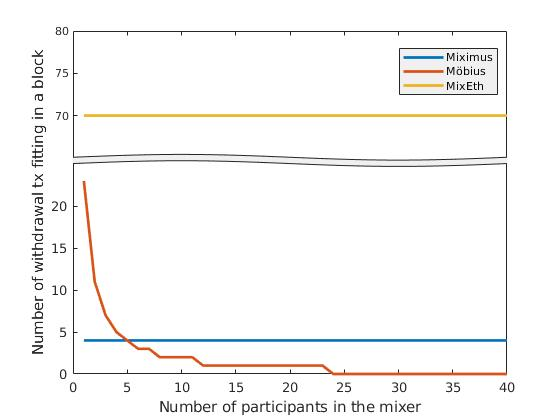
\includegraphics[scale=0.35]{./withdrawalComplexity.jpg}
	\captionsetup{justification=centering}
	\caption{Gas complexity of withdraw txs for various trustless Ethereum coin mixers}
\end{wrapfigure} 

\subsection{Withdrawing}
Let $C^*_{final}$ be the final shuffling accumulated constant. For a recipient $B$, whose public key $s_{B}G \in initPubKeys[]$, in the final shuffle there will be $s_{B}C^*_{final}$. The recipient can prove to MixEth that she knows secret key $s_{B}$ by signing their public key using a modified ECDSA, which uses $C^*_{final}$ as the generator element instead of the standardized $G$.

\section{Informal reasoning about security properties}

\begin{itemize}
\item \textbf{Recipient anonymity}
The withdrawing transaction for recipient $B$ sends funds to the public key $s_{B}C^{*}$. This public key does not reveal any links to the original $s_{B}G$ in case if at least one honest participant shuffled and the DDH assumption holds. Adversary can only distinguish between honest recipients public keys with negligible probability.
\item \textbf{Availability}
If an adversary is able to destroy an honest recipient's funds' availability, it implies that adversary $\adv$ either breaks the completeness of the Chaum-Pedersen protocol or successfully launched an eclipse attack against the honest recipient, who can not send any transactions to honest Ethereum peers.
\item \textbf{Theft prevention} 
If an adversary is able to steal funds from other users than it would imply that they managed to create a valid message/signature, $(m,\sigma)$ pair for the final shuffled public key of an honest recipient without having access to the secret key of the honest recipient. This contradicts to the assumption that ECDSA is existentially unforgeable. 
\end{itemize}
\section{Implementation}

We implemented MixEth in Solidity with two different approaches. The first one does not apply state channels, all the transactions are made on-chain. This could lead to unwanted gas costs as the number of corrupted shuffles increases. One of our main motivation with MixEth is to provide an efficient and scalable coin mixing protocol which uses as little blockchain resources, storage and gas, as possible. Therefore we also implement and evaluate MixEth applying state channels, namely shuffling and challenging a shuffle occurs off-chain and only deposit and withdrawal transactions happen on-chain.
Both of the implementations allow users to mix Ether or other ERC20-compatible tokens.

The bottleneck of coin mixing protocols is the withdrawal transactions' gas costs. A Miximus withdrawal transaction burns $\num[group-separator={,}]{1903305}$ gas, regardless of the number of participating parties. Since the block gas limit is $\num[group-separator={,}]{8000266}$ as of 2018, October 24 only 4 Miximus withdrawal transactions could fit in one Ethereum block. This is even worse for Möbius, since the gas cost for withdrawing coins from a Möbius mixer contract linearly increases with the numbers of participants.

\subsection{Fully on-chain implementation} \label{fullyonchainimpl}

Conceivably mixers would like to minimize off-chain coordination, therefore in our first implementation of the MixEth protocol, we assumed that all transactions will take place on-chain. There is only a single off-chain message from receiver to sender, where receiver delivers their public key to the sender. The rest of the protocol happens entirely on-chain.

On-chain storage is extremely expensive: it requires $\num[group-separator={,}]{20000}$ gas to store a $256$-bit number, however if a particular storage slot is already taken and one wants to overwrite it with a non-zero element than storing only consumes $\num[group-separator={,}]{5000}$ gas. To minimize on-chain storage costs, only the last two list of shuffled public keys are stored in the MixEth contract's permanent storage. Note that storing only the latest list of shuffled public keys would not be enough, since honest receivers could not prove to the contract that their shuffled public key is compromised unless also the last-but-one list of shuffled keys is also available for the contract to check the Chaum-Pedersen proof against. Such a storage structure implies that after uploading the new list of shuffled public keys, a challenging period should proceed in order to let receivers check the correctness of the shuffle and whether their shuffled public key is stored in the smart contract. Furthermore we also allow senders to shuffle and deposit new public keys at the same time, meaning that only $3$ on-chain transactions (shuffle, withdraw mixed coins and withdraw shuffling deposit) are sufficient to complete the protocol. We left it as a future work to determine the optimal ratio of mixed coins and shuffling deposits in order to incentivise correct shuffling.

A great advantage of the fully on-chain version of MixEth is that it allows dynamic anonymity sets. One could potentially deposit funds to the contract and shuffle public keys and leave funds in the mixing contract for indefinite amount of time. As soon as the anonymity set is large enough a receiver could withdraw their assets. A receiver in a MixEth contract with $N$ senders could withdraw their funds after $N^{'}$ shuffling rounds, where $N^{'}$ is arbitrary.  This dynamic nature of the contract could even lead to a single monolithic MixEth contract instead of having multiple MixEth contracts with significantly fragmented anonymity sets. A single MixEth contract is able to support the mixing of ether and ERC-20 compatible tokens as well. However note that the gas complexity of shuffling transactions grow linearly in the number of participants, therefore the fully on-chain implementation is not capable to support extremely large anonymity sets with participants more than cca. $\num[group-separator={,}]{800}$. 

Also note that the on-chain cost of a shuffle transaction could be amortized among participants. Specifically if there is a group of senders or receivers who trust each other they could collectively charge any of them to shuffle once. Since they trust their peer, all the rest of the group does not need to shuffle anymore. Later non-shufflers could reimburse the only shuffler for their services either on-chain or off-chain. 
        
\subsection{State channel implementation} \label{statechannelimpl}

We have also adapted MixEth to operate within a state channel. We wrote the implementation within the guidelines of the Counterfactual framework \cite{coleman2018counterfactual}. This allowed us to delegate the processes of setup, liveness disputes and finalisation to the framework so that we could focus on adapting the application logic. Unlike the on-chain implementation the state channel implementation requires that the set of participants be agreed upon upfront. In state channels each update to the state needs to be signed by all other participants, this means that state channel applications are inherently at least $\mathcal{O}(n)$. To co-ordinate these off-chain updates the Counterfactual framework enforces that all applications be turn based, introducing a turn taker for each turn who may propose a new state. The original MixEth implementation was not turn based so we have adapted the application to this constraint, an example of this adaptation is the challenge round. In the on-chain implementation a time period is allowed during which any participant may challenge, we have adapted this by proceeding turn-based through the participants offering each the chance to either challenge or pass. In the case of a breakdown in cooperation in the channel, a liveness fault, it has been shown that all operations succeeding the cooperation breakdown must proceed on chain\cite{mccorryyou} or be abandoned at some financial cost specified by the application, meaning that if every shuffle were to be succeeded by a challenge round each participant would be forced, by threat of lost deposit, to make an on-chain transaction after each shuffle, incurring $\mathcal{O}(n)$ on chain operations. To mitigate this we removed the challenge after each round and instead introduced a challenge round that takes place after all shuffles have completed, during this round any of the preceding shuffles may be challenged.

Given these adaptations the application proceeds as follows, all participants including senders, shufflers and receivers, deposit funds in a mutli-signature wallet compatible with the Counterfactual framework, they then follow the installation protocols specified by the framework to install the adapted MixEth logic. Afterwards each participant signs a transaction that transfers an equal amount to each withdrawer from the multi-sig, dependent on correct execution of the channelised MixEth application logic. This application logic proceeds as follows: each sender names a public key of a shuffler as in the deposit stage of the on-chain application, then each shuffler takes it in turn to shuffle. After all shuffles have taken place each withdrawer is given a turn to either declare fraud or no-fraud on any shuffle round. Finally each withdrawer then provides proof of ownership by submitting a valid signature on the modified ECDSA scheme. 

If any of these steps does not occur, or does not occur correctly, the protocol aborts and the conditional transfer does not occur. In this case the perpetrator loses a deposit, either through fraud proof or through failure to take their turn when state is published on-chain. A further modification would be to distribute the slashed deposit to each of the other participants, compensating them for their lost time and the gas costs associated with proving the fault of the other party. 

Following this protocol the on-chain transactions are now reduced to: one transaction from each participant to deposit funds into the multi-sig, and a set of transactions that send funds from the multi-sig to each of the withdrawers and deposits back to each of the other participants. 

\begin{table}[H] 
	\caption{Proof-of-concept implementation gas cost results. MixEthChannel refers to the implementation which leverages state channels for shuffling and challenging periods}
	\centering 
	\begin{tabular}{@{\extracolsep{6pt}}lccccc@{}} 	
		\toprule
		\hline
		&Deployment&Deposit&\multicolumn{2}{c}{Shuffle}& Withdraw\\
		\cline{4-5}&&&Shuffle upload&Challenge\\
		\hline
		\midrule
		Möbius \cite{meiklejohn2018mobius}     &$\num[group-separator={,}]{1046027}$&$\num[group-separator={,}]{76123}$&0&0&$\num[group-separator={,}]{335714}$n   \\
		Miximus \cite{miximus2018}&$\num[group-separator={,}]{1751378}$&$\num[group-separator={,}]{732815}$&0&0 &$\num[group-separator={,}]{1903305}$  \\
		MixEth&TBD&$\num[group-separator={,}]{99254}$&$\num[group-separator={,}]{138653}+\num[group-separator={,}]{10000}n$&$\num[group-separator={,}]{227563}$&$\num[group-separator={,}]{113265}$  \\
		MixEthChannel&TBD&TBD&0&0&TBD\\
		\bottomrule
	\end{tabular}
	\label{table:gasproperties}
\end{table} 
\newpage
\bibliographystyle{plain}
\bibliography{sample}

\end{document}
